\documentclass[aps,prl,reprint]{revtex4-1}
\usepackage{blindtext}

\usepackage{amsmath}
\usepackage{graphicx}
\usepackage{commath}
\usepackage{siunitx}
\usepackage{tabularx}

\usepackage{graphicx}




\usepackage[b]{esvect}

\newcommand{\de}{\mathrm{d}}

\usepackage{longtable}
\graphicspath{ {images/} }
\begin{document}
\title{Unit 1: Instruments, Signals, Resistors}
\author{Xueqi Li}
% \email{xueqi.li@stonybrook.edu}
\thanks{Partner: Tianming Hai}
% \author{partner Tianming Hai}
\noaffiliation
\date{Feb 10, 2019}


% \begin{abstract}
% Here I tell what I have done... And I have done a lot but it is hard to tell what exactly I have done...
% \end{abstract}

\maketitle

\section{Introduction}  
    \subsection{Digital Multi-meters}
    
    The digital multi-meters is used when one want to measure the resistance, current, or voltage. It has buttons to switch to different function to measure different quality, and use another set of buttons to change the maximum value can be measure (and the unit sometime). To appropriately plug it into the circuit, different port on the multi-meters might be used. For our case, resistance and voltage share same port but current use a different port with two different maximum acceptable current. Once pluging into the circuit, One may read the digit on the screen of the meters to find the value of resistance, current, or voltage. It is importent to make sure the current is smaller than the maximum acceptable current of the meters. For unknow current, usually use the larger maximum port first.

        \subsubsection{Root Mean Square}
        When measure a changeing voltage with the voltagemeter mode. The metter gives a root mean square value:
        \[
            V_{\text{rms}} = \sqrt {\frac{1}{T} {\int_{t}^{t + T} {[V(t)]}^2\, dt}}
        \]
        For example, when giving a sine wave ($V(t) = V_0 \sin(\omega t)$), the reading would be $\frac{V_0}{\sqrt{2}}$. When giving a triangle wave in a amplitude of $V_0$, the reading would be $\frac{V_0}{\sqrt{3}}$. And the reading of square wave would be its origina amplitude.


    \subsection{Oscilloscope}
    A oscilloscope is used when measure the voltage. The oscilloscope can output a plot of voltage versus time so that one may identify the changes of voltage. To use a oscilloscope, one may plug two channel in to the circuit to measure the voltage of two different parts of the circuit. Once the scope been appropriately pluged into the circuit, one may use knobs on the scope to change the scale and position of the plot. Once the plot has been appropriate display on the screen, a measure button might be useful to read the accurate value of voltage, frequency, or other useful quality. One may use a the dual mode under the display menu to display a plot of voltage of channel 1 versus voltage of channel 2.

    Usually the oscilloscope measure function can give you the maximum value of the input voltage.

    \subsection{Signal Generator}
    A signal generator is used when the input voltage is required to be a sine wave, a square wave, or a triangle wave. One can use the form button to change between those wave form. To change the frequency, use the numberpad and the unit button. It is also possible to chagne the amplitude by using the amplitude knobs.

    \subsection{Grounded}
    A importent principle of using those devices is to notice that the outer shell is connected to the ground. Thus, the outer shell of different devices are connected together. It is a good idea to keep all outer shell connect at the same point of the circuit so that it does not affect the circuit.

    \subsection{Jobboard}
    The board is useful to connect the circuit. The board which is used in this lab have two different layout. The first one is the long panel where the width is two port. Such panel connected the port in column together and marked as red and blue lines. The other one have width as five port. Such panel connected the port in rows together.

    One may use wires and ohmmeter to identify which of two ports are connected. The open circuit gives the meter no reading (blinking zero), and the connected ports will give meter a small reading.

    One may use wire stripper or precut jumpers to help the layout of the circuit on the board. To use the wire stripper, one can cut the wire or strip the insulation shell of the wire. A precut jumpers can be used to connect different part of the board into one.

    \subsection{Resistor Bar Code}
        \begin{table}
        \begin{ruledtabular}
        \begin{tabular}{ccc} 
        Color & Significant digits & Multiplier\\
        \hline
        \hline
        Black & 0 & $10^0$ \\ 
        \hline
        Brown & 1 & $10^1$ \\
        \hline
        Red & 2 & $10^2$ \\
        \hline
        Orange & 3 & $10^3$ \\
        \hline
        Yellow & 4 & $10^4$ \\ 
        \hline
        Green & 5 & $10^5$ \\ 
        \hline
        Blue & 6 & $10^6$ \\ 
        \hline
        Violet & 7 & $10^7$ \\ 
        \hline
        Grey & 8 & $10^8$ \\ 
        \hline
        White & 9 & $10^9$ \\ 
        \end{tabular}
        \end{ruledtabular}
        \caption{Color code for resistance value}
        \label{table:1}
        \end{table}
    A resistor bar code can give useful information of the resistor such as its resistance. One may refer to Table~\ref{table:1} to find its resistance.
    \subsection{Resistor}
    A resistor follows Ohm's law linearly:
    \[
    R = \frac{V}{I}
    \]
    If we connect two resistor in series, they would share same current but occupied different voltage. One may find:
    \[
    R_\text{total} = R_1 + R_2
    \]
    If we connect two resistor in parallel, they would share same current but use different current. One may find:
    \[
    \frac{1}{R_\text{total}} = \frac{1}{R_1} + \frac{1}{R_2}
    \]
    \subsection{Ohmmeter}
    The lab is using a GDM-8145 multi-meter. When using as a ohmmeter, it will apply $0.2V$ or $2V$ on the resistor\cite{dmm}. The current passed through the resistor is given as $I = \frac{V}{R}$.
    \subsection{Ohm's Law}
    A conductor usually have some electric conductirity:
    \[
    \sigma = \frac{1}{\rho}
    \]
    Where $\rho$ is resistivity of the material. Usually the conductirity is a constent, this imply the Ohm's law:
    \[
    \vv{J}(\vv r) = \sigma \vv E (\vv r)
    \]
    Thus, one may find the current:
    \[
    I = \int \vv J \cdot \de \vv A
    \]
    where the integral is over the cross section. One may also find the voltage as:
    \[
    V = - \int \vv E \cdot \de \vv l
    \]
    This give us the resistance:
    \[
    R := \frac{V}{I}
    \]

    \subsection{Measuring Resistance with a Scope}
    \begin{figure}[h]
        \centering
        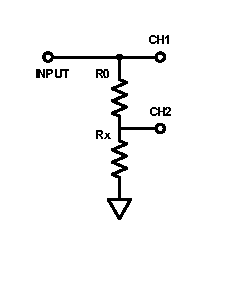
\includegraphics{images/plot1.pdf}
        \caption{Circuit of resistance measurement}
        \label{fig:1}
    \end{figure}
    One may measure the resistance of a resistor by using circuit in Figure~\ref{fig:1}. Where $R_0$ is some knowning resistor with a large resistance. To find the resistance, one may wish to find the current and the voltage on the unknow resistor. Here, channel 1 measure the current:
    \[
    I = \frac{V}{R_\text{total}} = \frac{V}{R_0 + R_x} \approx \frac{V}{R_0}
    \]
    This approxmation is able to use since $R_0$ is much larger than $R_x$

    Once the current is found, one can calculate the resistance:
    \[
    R = \frac{V_\text{CH2}}{I} = \frac{V_\text{CH2}R_0}{V_\text{CH1}}
    \]
    It is easy to see that the a plot of voltage of channel 2 versus voltage of channel 1 is useful, One may use the dual mode of the scope to output such plot and find $\frac{V_\text{CH2}}{V_\text{CH1}}$ as the slope.
    \subsection{Voltage Divider}
    \begin{figure}[h]
        \centering
        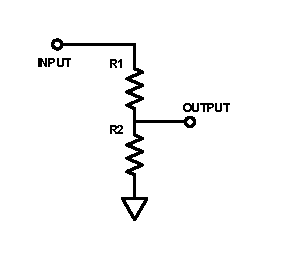
\includegraphics{images/plot2.pdf}
        \caption{A voltage divider}
        \label{fig:2}
    \end{figure}
    A voltage divider is form by the circuit of Figure~\ref{fig:2}. One may find the current is given as:
    \[{}
    I = \frac{V_\text{in}}{R_\text{total}} = \frac{V_\text{in}}{R_1 + R_2}
    \]
    Thus, the voltage on $R_2$, which is also the output voltage, is given as:
    \[
    V_\text{out} = V_2 = IR_2 = \frac{V_\text{in} R_2}{R_1 + R_2}
    \]

    Thus, one may also find from above equation
    \[
    \frac{V_\text{out}}{V_\text{in}} = \frac{R_2}{R_1 + R_2}
    \]
    For example, to have a $1:10$ divider, it is nesseary to have $R_1 = 9R_2$. To have a $1:5$ divider, it is nesseart to have $R_1 = 4R_2$
        \subsubsection{Voltage Divider and Other Device}
        Many device have a build-in resistor. Thus, when using them with other resistor, sometimes it forms a voltage divider and affect the measurement. For example, the signal generator in lab have a $50\Omega$ build-in resistor. It is nesseary to use a large resistor in the circuit to avoid the influences of the build-in resistor.
    \subsection{Decibel Unit}
    The Decibel (dB) is a logarithmic unit defined by:
    \[
    G_\text{dB} = 20 \log_{10}(\frac{V_0}{V})
    \]
    For example, if given $V_0$ as 1V, than 1V is 0dBV, 10V is 20dBV, 1mV is -60dBV.
    \subsection{Thevenin's equivalents}
        \begin{figure}[h]
        \centering
        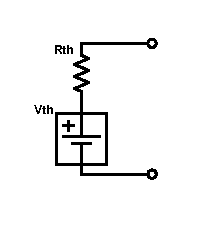
\includegraphics{images/plot5.pdf}
        \caption{Thevenin's equivalents}
        \label{fig:5}
    \end{figure}
    Thevenin's theorem suggest that any linear electrical circuit with voltage sources and resistances have a equivalent circuit with one voltage sources and one resistor in series as present in Figure~\ref{fig:5}. One may construct such equivalent circuit by finding the equivalent voltage $V_\text{th}$ and the equavalent resistor $R_\text{th}$.

    To find the equivalent voltage and resistor, one can measure the voltage and the current of the output of the circuit. The equavalent voltage is juat as same as measured voltage and the equavalent resistor can be find by Ohm's law as $R_\text{th} = \frac{V}{I}$. However, it is not safe to direct plug the ammeter on the output since the output current might be very large and damage the ammeter. One may use a load resistor parallel with a voltmeter to find the equavalent resistor. Consider the whole circuit as a voltage divider, the output of the voltmeter follows equation:
    \[
    V = \frac{V_\text{th} R_\text{L}}{R_\text{th} + R_\text{L}}
    \]
    Thus we can find the equavalent resistor have resistance as:
    \[
    R_\text{th} = \frac{V_\text{th}R_\text{L}}{V} - R_L
    \]
\section{Data}
    \subsection{DC Power}
    One may measure the voltage of a DC power supply. The reading from the DMM is $5.05\pm0.01$V, and the reading from oscilloscope is $5.02\pm0.25$V.
    \subsection{Resistor}
    \begin{table}[h]
    \begin{ruledtabular}
    \begin{tabular}{cccc} 
    Resistor & Code bar [$\Omega$] & Measurement [$\Omega$] & Difference \\
    \hline
    \hline
    $R_1$ & $3.3 \times 10^4$ & $3.35(1)\times 10^4$ & 1.52(1)\% \\ 
    \hline
    $R_2$ & $1.0 \times 10^3$ & $1.10(1)\times 10^3$ & 10.00(1)\%\\
    \hline
    $R_3$ & $1.10 \times 10^4$ & $1.106(1)\times 10^4$ & 0.54(1)\%\\
    \end{tabular}
    \end{ruledtabular}
    \caption{Code bar reading and the real value}
    \label{table:2}
    \end{table} 
    A resistor might have different resistance from its bar code. Please find the measument and the bar code reading in the Table~\ref{table:2}.

    \begin{figure}[h]
        \centering
        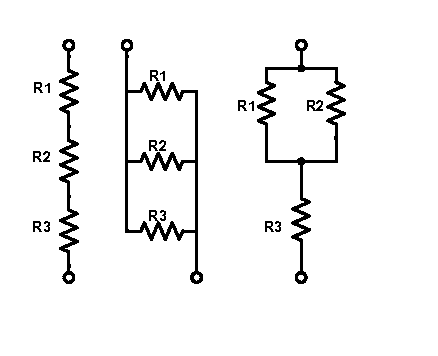
\includegraphics{images/plot3.pdf}
        \caption{Series, parallel, and series-paralel from left to right}
        \label{fig:3}
    \end{figure}
    One can also form a circuit to connect those resistor in series, parallel, and series-paralel as in Figure~\ref{fig:3}.
    \begin{table}[h]
    \begin{ruledtabular}
    \begin{tabular}{cccc} 
    Circuit & Theoretical [$\Omega$] & Measurement [$\Omega$]\\
    \hline
    \hline
    Series & $4.57(5)\times 10^4$ & $4.60(1)\times 10^4$\\ 
    \hline
    Parallel & $9.71(1) \times 10^2$ & $9.72(1)\times 10^2$\\
    \hline
    Series-parallel & $1.17(10)  \times 10^4$ & $1.21(1)\times 10^4$\\
    \end{tabular}
    \end{ruledtabular}
    \caption{Series or parallel of resistor}
    \label{table:3}
    \end{table} 
    We can measure the resistance in each case as in Table~\ref{table:3}. To find the theoretical value of the resistor, we can proceed following computation:
    \begin{enumerate}
        \item Series:
        \begin{align*}
            R &= R_1 + R_2 + R_3 = 4.57\times 10^4 \Omega \\
            \sigma_R &= \sqrt{\sum (\frac{\partial R}{\partial R_i})^2\sigma_{R_i}^2} = 0.05\times 10^4 \Omega\\
        \end{align*}
        \item Parallel:
        \begin{align*}
            R &= \left(\frac{1}{R_1}+\frac{1}{R_2}+\frac{1}{R_3}\right)^{-1}\!\!\!\!\!\! = 9.71 \times 10^2 \Omega\\
            \sigma_R &= \sqrt{\sum (\frac{\partial R}{\partial R_i})^2\sigma_{R_i}^2} = 0.01 \times 10^2 \Omega
        \end{align*}
        \item Series-parallel:
        \begin{align*}
            R &= \left(\frac{1}{R_1}+\frac{1}{R_2}\right)^{-1}\!\!\!\!\!\! + R_3 = 1.17 \times 10^4 \Omega\\
            \sigma_R &= \sqrt{\sum (\frac{\partial R}{\partial R_i})^2\sigma_{R_i}^2} = 0.10 \times 10^4 \Omega
        \end{align*}
    \end{enumerate}
    By reconnected the resistor, we find the board connection have a small resistance.

    \subsection{Measure resistance using scope}
    To measure the unknown resistance as in the introduction, We use a load resistor with resistance $3.35(1)\times 10^4 \Omega$, and obtained a plot with slope of $k = \frac{0.15(1)\text{V}}{5.0(5)\text{V}} = 0.030(3)\text{V}$. Thus we have $R_x = kR_0 = 1.01(10)\Omega$. The real value of the resistor is $1.10(1)\times 10^3\Omega$ by measument.

    \subsection{Voltage divider}
    To achieve a 1:10 voltage divider, we use $R_1$ as three resistor in series to have a $5200\Omega+3670\Omega+150\Omega = 9020\Omega$ resistance, and we use a $1000\Omega$ as $R_2$. In measurement with a scope, we find the image coincide when we use the input channel in a scale of 1V and the output channel in a scale of 100mV. This is indeed a 1:10 voltage divider. The error is the half of the minimum scale (10mV). When apply a DC power of 15.00(1)V, we find the output is 1.49(1)V.


    \begin{table}[h]
    \caption{Output and Input for voltage divider}
    \begin{ruledtabular}
    \begin{tabular}{ccc} 
    \multicolumn{3}{c}{Sine Wave Set 1} \\ \hline\hline
    Input Frequency & Output Voltage{[}mV{]} & Output Frequency \\ \hline\hline
    100Hz           & 204(4)                 & 100.0(1)Hz       \\ \hline
    1kHz            & 204(4)                 & 1.00(5)kHz       \\ \hline
    500kHz          & 200(1)                 & 500(1)kHz        \\ \hline
    700kHz          & 192(4)                 & 700(2)kHz        \\ \hline
    1MHz            & 176(4)                 & 1.00(1)MHz       \\ \hline
    2MHz            & 128(4)                 & 2.00(1)MHz       \\ \hline
    3MHz            & 92(4)                  & 3.00(2)MHz       \\ \hline
    4MHz            & 72(4)                  & 4.00(5)MHz       \\ \hline
    5MHz            & 56(4)                  & 5.00(5)MHz       \\ \hline
    10MHz           & 28(4)                  & 10.00(1)MHz      \\ \hline\hline
    \\
    \multicolumn{3}{c}{Sine Wave Set 2} \\ \hline\hline
    Input Frequency & Output Voltage{[}mV{]} & Output Frequency \\ \hline\hline
    100Hz           & 100(4)                 & 100(2)Hz         \\ \hline
    1kHz            & 100(4)                 & 1.00(3)kHz       \\ \hline
    5kHz            & 100(1)                 & 5.00(1)kHz       \\ \hline
    1MHz            & 88(4)                  & 1.00(2)MHz       \\ \hline
    5MHz            & 42(4)                  & 5.00(5)MHz       \\ \hline
    9MHz            & 36(4)                  & 8.95(5)MHz       \\ \hline\hline
    \\
    \multicolumn{3}{c}{Triangle Wave} \\\hline\hline
    Input Frequency & Output Voltage{[}mV{]} & Output Frequency \\ \hline\hline
    100Hz           & 100(4)                 & 100(2)Hz         \\ \hline
    1kHz            & 100(2)                 & 1.00(2)kHz       \\ \hline
    5kHz            & 100(2)                 & 5.00(5)kHz       \\ \hline
    1MHz            & 74(2)                  & 1.00(5)MHz       \\ \hline\hline
    \\
    \multicolumn{3}{c}{Square Wave} \\\hline\hline
    Input Frequency & Output Voltage{[}mV{]} & Output Frequency \\ \hline\hline
    100Hz           & 100(2)                 & 100.0(3)Hz       \\ \hline
    1kHz            & 100(2)                 & 1.00(5)kHz       \\ \hline
    5kHz            & 100(4)                 & 5.00(5)kHz       \\ \hline
    1MHz            & 100(2)                 & 1.00(2)MHz       \\ \hline
    5MHz            & 66(2)                  & 5.00(3)MHz       \\ \hline
    9MHz            & 48(2)                  & 9.0(1)MHz        \\ 
    \end{tabular}
    \footnotetext{The input voltage is 2V for each measurement on sine wave set 1. The input voltage is 1V for each of other measurement.}
    \footnotetext{Two set of result of sine wave are perform in different date.}
    \end{ruledtabular}
    \label{table:4}
    \end{table} 
    When using different frequency in the input from the signal generator, we obtained ths result as in Table~\ref{table:4}.

    \subsection{Signal Generator}
    When set the signal generator to 100Hz, we see the result on the scope is 100(2)Hz when they are connected directly.

    \subsection{Phase shift}
    \begin{table}[h]
    \begin{ruledtabular}
    \begin{tabular}{ccc} 
    Input & Time Difference [ns] & Phase Shift\\
    \hline
    \hline
    1MHz & 65.0(75) & 0.498(5)\\ 
    \hline
    2MHz & 77.5(75) & 0.817(9)\\
    \hline
    3MHz & 52.5(50) & 1.225(14)\\
    \end{tabular}
    \end{ruledtabular}
    \caption{Phase shift of a voltage divider}
    \label{table:5}
    \end{table} 
    One can measure the phase shift between the output and input of a voltage divider as in the Table~\ref{table:5}. To calculate the phase shift, we use $\Delta \varphi = \frac{\Delta t}{T} 2\pi$ where $T = \frac{1}{f}$. The phase shift before 500kHz is unrecognizable.

    \subsection{Root Mean Square}
    \begin{table}[h]
    \begin{ruledtabular}
    \begin{tabular}{cccc} 
    Waveform & Frequency & Scope{[}mV{]} & DMM{[}mV{]} \\ \hline\hline
    Sine     & 100Hz     & 204(4)        & 56(1)       \\ \hline
    Square   & 100Hz     & 212(2)        & 211(5)      \\ \hline
    Triangle & 100Hz     & 200(1)        & 57(1)       \\ \hline
    Sine     & 1kHZ      & 204(4)        & 57(1)       \\ \hline
    Square   & 1kHZ      & 206(4)        & 230(1)      \\ \hline
    Triangle & 1kHZ      & 200(2)        & 57(1)       \\ \hline
    Sine     & 100kHz    & 208(4)        & 27(1)       \\ \hline
    Square   & 100kHz    & 220(4)        & 254(5)      \\ \hline
    Triangle & 100kHz    & 200(4)        & 38(1)       \\ \hline
    Sine     & 1MHz      & 148(4)        & 57(1)       \\ \hline
    Square   & 1MHz      & 196(4)        & 507(1)      \\ \hline
    Triangle & 1MHz      & 124(4)        & 58(1)       \\ 
    \end{tabular}
    \end{ruledtabular}
    \caption{Difference between maximum value and RMS value}
    \label{table:6}
    \end{table} 
    One can measure the maximum value of a waveform by using a scope, or measure a RMS value using a DMM. A result is present in the Table~\ref{table:6}

    \subsection{Decibels}
    \begin{table}[h]
    \begin{ruledtabular}
    \begin{tabular}{ccc} 
    Before[V] & After[mV] & Theoretical[V] \\ \hline\hline
    4.0(2)    & 400(4)    & 0.4            \\ \hline
    6.0(2)    & 720(4)    & 0.6            \\ \hline
    8.0(2)    & 1000(40)  & 0.8            \\ \hline
    10.0(2)   & 1200(40)  & 1.0              \\
    \end{tabular}
    \end{ruledtabular}
    \caption{Before and after change the dB setting}
    \label{table:7}
    \end{table} 
    The -20dB setting on the signal generator can change the amplitued. This setting will theoreticaly reduced the amplitued to its $\frac{1}{10}$ of origina. A data obtained before and after using the dB setting is present in Table~\ref{table:7}

    \subsection{Thevenin's Equivalents}
    One can form a 1:2 voltage divider with a 15 V voltage sources and find its equivalent. By measurement, we find the output is 7.60(4)V and 14.9(1)mA, this give us the equivalent voltage as 7.60(4)V and the equivalent resistor is 510.07(5)$\Omega$. We can calculated the theoreticaly equivalent resistor as following:
    \begin{align*}
        R_\text{th} &= \frac{V_2}{I_\text{no2}} = \frac{R_2I}{\frac{V_\text{in}}{R_1}} = \frac{R_2 \frac{V_\text{in}}{R_1 + R_2}}{\frac{V_\text{in}}{R_1}} = 500\Omega \\
        V_\text{th} &= V_2 = R_2 \frac{V_\text{in}}{R_1 + R_2} = 7.5V
    \end{align*}


    \subsection{Load Resistor}
    \begin{table}[h]
    \begin{ruledtabular}
    \begin{tabular}{cccc} 
    Load[k$\Omega$] &  Output Voltage[V] & $R_\text{th}[\Omega]$ & Theoretical Voltage\\ \hline\hline
    50              & 0.680(1)           & 501(1)                & 0.682 \\ \hline
    500             & 3.75(1)            & 500(1)                & 3.75 \\ \hline
    5000            & 6.80(1)            & 514(1)                & 6.82 \\
    \end{tabular}
    \end{ruledtabular}
    \caption{Load resistor and the output}
    \label{table:8}
    \end{table} 
    One may also apply a load resistor to the output and find the equivalent resistor. A measurement is as Table~\ref{table:8}. To find the equivalent resistor, one can apply
    \begin{align*}
        R_\text{th} &= \frac{V_\text{th}R_L}{V} - R_L\\
        \sigma_{R_\text{th}} &= \sqrt{(\frac{\partial R_\text{th}}{\partial R_L})^2\sigma_{R_L}^2+(\frac{\partial R_\text{th}}{\partial V})^2\sigma_{V}^2}
    \end{align*}


    \subsection{Series and Parallel}
    \begin{figure}[h]
        \centering
        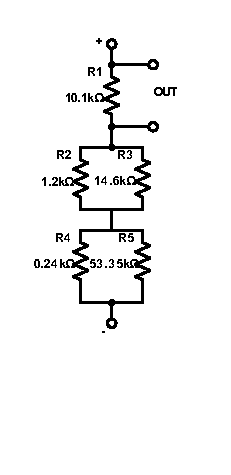
\includegraphics{images/plot4.pdf}
        \caption{Series and Parallel Resistors}
        \label{fig:4}
    \end{figure}
    One can use different resistors to form a series and parallel circuit. A such circuit is presented in Figure~\ref{fig:4} with a input 15V DC. We can pick a output point and measure the equavalent circuit. In measurement, we find the voltage is $12.936(5)$V and the current is $12.61(5)$mA. We may refer it as Figure~\ref{fig:5} to find the equavalent voltage is 12.936(5)V and the equavalent resistor is $1.025(6)k\Omega$ The theoretical value of equavalent reisitor can be calculate to be $1.009k\Omega$.

\section{Analysis}
    \subsection{DC Power}
    The result is reasonable. The DC power gives around 5V voltage and the result in DDM and scope agrres in $2\sigma$.
    \subsection{Resistor}
    The result is reasonable. Most of the resistor have a less than 2\% difference than its color bar. One resistor have difference in 10\%. This resistor might needed to be replaced from the lab.

    For series and parallel those resistor, the theoretical value and the measurement value are closed. The measurement value is a little bit larger than the theoretical value, that might be due to the resistor on wire.
    \subsection{Measure resitance using scope}
    The resulted vlaue and the theoretical value agrees each other within $1\sigma$.
    \subsection{Voltage divider}
    We do achieve a 1:10 voltage divider. We find that in high frequency, the output voltage dorped in all waveform, which is not as expected in theory. It is true that the maximum input voltage did not change, it might be the case that the resistance is not truly linear in high frequency, or some voltage might be expend when it translate in wire in high frequency.
    \subsection{Signal Generator}
    The signal generator is capable to generate asking frequency within $1\sigma$.
    \subsection{Phase shift}
    For higher frequency, we see a phase shift in the output. Higher the frequency, higher the phase shift. It might be the case that the current have a delay since it takes time to transmit to the output channel.
    \subsection{Root Mean Square}
    The result is not reasonable. We see that in square wave, low frequency gives a reasonable result (RMS is equal to maximum). However, in high frequency, it does not gives a reasonable result. It might be the case that when high frequency, the signal generator cannot generate a well square wave sometimes. The wave form might be decompose into dispersed sin wave given by Fourier transform, thus it gives a none reasonable result. For sine and triangle wave, it does not gives reasonable result at all. As in the introduction part, the result of the sine wave shoule be $\frac{V_\text{max}}{\sqrt{2}}$ and the result of the triangle wave should be $\frac{V_\text{max}}{\sqrt{3}}$. There might be a operation error.

    \subsection{Decibels}
    The result is not very well. The result value is close to the theoretical value but higher. That might be a defect on signal generator.
    \subsection{Thevenin's Equivalent}
    The result is reasonbale. The theoretical value and the resulted value are clossed but the resulted value is higher. That might be due to the resistance of wire.
    \subsection{Load resistor}
    The result is reasonable. We see that the load resistor closed to the equavalent resistor gives more precise value.

    \subsection{Series and Parallel}
    The result is reasonable. The theoretical value and the resuted value are within $2\sigma$.

    One may ask for such circuit, how does the load resistor affect the result value. We can think such cirrent as a voltage divider (think $R_2$, $R_3$, $R_4$, and $R_5$ as one resistor $R_1$ in voltage divider and the origina $R_1$ is $R_2$ in voltage divider). One can find by dirrect measument, the equavalent resistance can be find by
    \[
    R_\text{Dth} = \frac{V_2}{I_\text{no2}} = \frac{V_\text{in} R_2}{R_1 + R_2} \frac{R_1}{V_\text{in}} = \frac{R_1R_2}{R_1+R_2}
    \]
    However, when we using a load resistor, we can find 
    \begin{align*}
        R_\text{Lth} &= \frac{V_\text{th} R_L}{V_L} - R_L \\
        &= \frac{V_\text{in} R_2 R_L}{R_1+R_2}
        \frac{ R_1+(\frac{1}{R_L} + \frac{1}{R_2})^{-1}}
        {V_\text{in}} (\frac{1}{R_L} + \frac{1}{R_2}) - R_L\\
        &= \frac{R_2 R_L (R_1+(\frac{1}{R_L} + \frac{1}{R_2})^{-1})}{R_1+R_2} (\frac{1}{R_L} + \frac{1}{R_2}) - R_L
    \end{align*}
    Now we can see that the dirrect measurement is not depend on the anything but the loaded measurement is depend on the load resistor. We can use the equation to find when would the the the load resistor make the result have more error. After a calculation, even $1M\Omega$ is still within the 10\% range for this circuit.

\section{Conclusion}
Overall the result is reasonable. However, the root mean square part have a serious error. This might due to a operation error, or the wire connected to the DMM have some problem. In the last part, maybe it is nesseary to view the equation in a log scale.

\bibliography{cite}
\bibliographystyle{apsrev4-1}

% \begin{center}
%  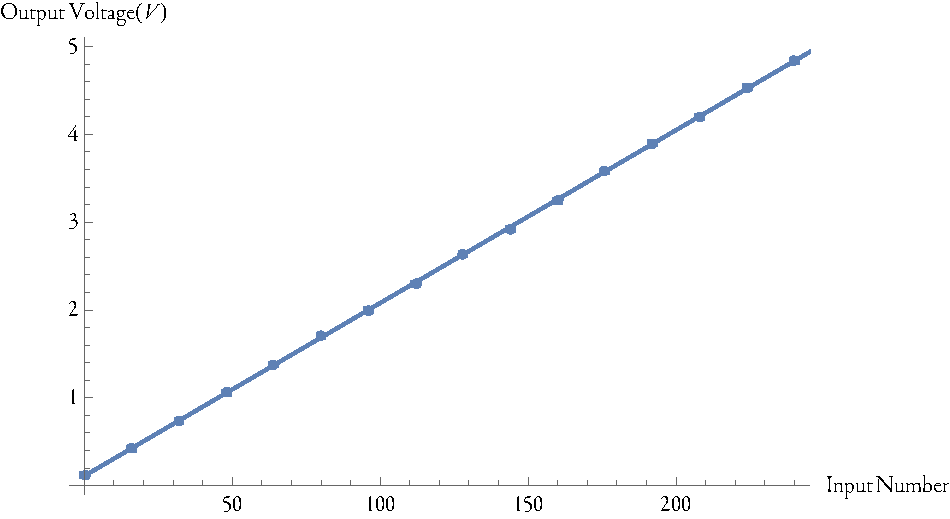
\includegraphics[height=1.8in]{plot.pdf}
% \end{center}

%\begin{center}
% 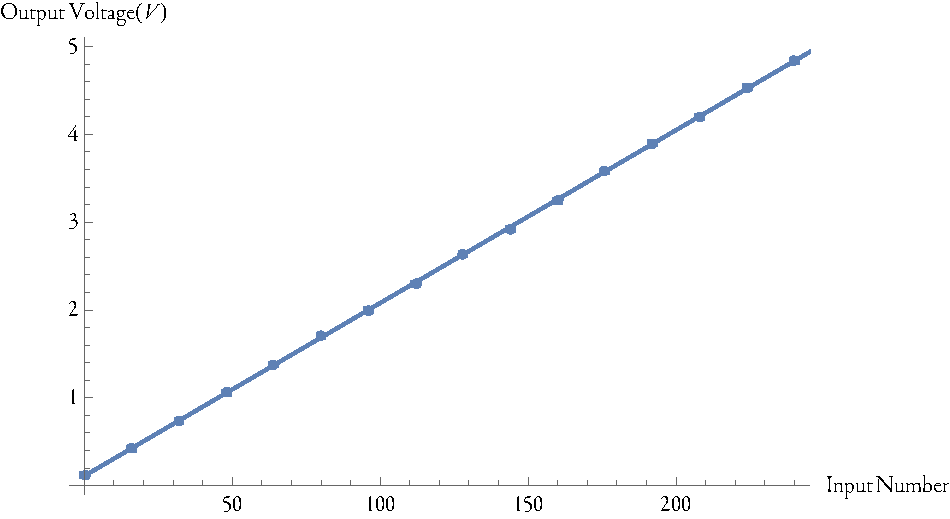
\includegraphics[height=1.3in]{plot.pdf}
%\end{center}

% \blindtext \cite{article-minimal}

% \bibliographystyle{apsrev4-1} % Tell bibtex which bibliography style to use
% \bibliography{xampl} % Tell bibtex which .bib file to use (this one is some example file in TexLive's file tree)

\end{document}